\subsection{Kubernetes Installation}
The Kubernetes master installation in the cloud is well documented and did not pose any trouble. For completion of this thesis I will briefly mention the additional components installed on the master. Kubernetes has no default networking implementation, I thus installed Flannel\cite{coreosFlannel:online}, one of the simplest and most widely used networking fabrics specifically designed for Kubernetes. It runs a small binary called \textit{flanneld} on each node and provides networking between nodes and pods\footnote{The specifics of Flannels networking are outside this thesis scope, for more information see \url{https://blog.laputa.io/kubernetes-flannel-networking-6a1cb1f8ec7c}}. For administrative purposes I also installed the Kubernetes Dashboard However, the Raspberry Pi Foundation recently released a update to Raspbian called buster, which does not support the aufs-dkms kernel modules anymore, which are dependencies of kubeadm and docker. Online, the community advised to avoid the dependency but if possible switch back to the older version of raspberian called stretch. Out of time concerns, I switched back to the old version. In the future I plan to use containerd instead of docker, which could these problems and more\footnote{Containerd is only the container runtime. Compared to Docker CE it has less features but is faster and uses less memory.}.\\
I also switched the official Kubernetes kubelet with the kubelet binary from Ranchers K3s called Hyperkube. \Cref{fig:kubeBinaries} shows the size of the binary files of three most important components of Kubernetes, kubeadm, kubelet and kubectl.
\begin{figure}[h!]
    \centering
    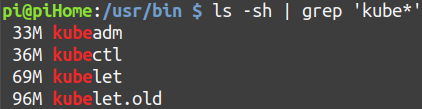
\includegraphics[scale=0.5]{figures/kubeBinariesSize.png}
    \vspace*{-0.3cm}
    \caption{The sizes of the kubernetes binaries.\\ Note, \textit{kubelet} is the K3s hyperkube binary and \textit{kubelet.old} is the official kubelet bianry.}
    \label{fig:kubeBinaries}
\end{figure}
In total the official binaries are 165 megabyte large and the kubelet (\textit{kubelet.old} file) takes almost half the space. Using the K3s build of kubelet (\textit{kubelet} file) brings the total amount to 138 megabyte saving almost 20\% of space in addition to its other benefits discussed in \cref{sec:kubelet} \nameref{sec:kubelet}. The full installation procedure can be found in the repository of this thesis for replication and validation.\\
Finally, the effects on the system resources are two folds, the native applications and the running containers. The Raspberry Pi has 926MB total memory and a 1.4 GHz quad-core CPU. Firstly, \cref{fig:kubernetesResourceConsumption} shows the resource usage of the native applications
\begin{figure}[h!]
    \centering
    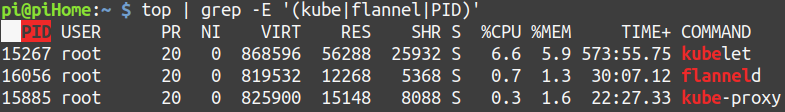
\includegraphics[scale=0.5]{figures/kubernetesResourceConsumption.png}
    \vspace*{-0.3cm}
    \caption{ The resource usage of native Kubernetes components (using K3s hyperkube binary).}
    \label{fig:kubernetesResourceConsumption}
\end{figure}
The kubelet process uses 6.6\% of the CPU and 5.9\% of the memory\footnote{While the memory usage is consistent, the CPU usage varies a lot and can reach peaks of 16\%.}. Flanneld and kube-proxy both use less than 1\% CPU and 1.3\% and 1.6\% of memory, respectively. It is important to note that the container runtime is not included in that statistics. The resource usage of the containers is shown in \cref{fig:kubernetesResourceConsumptionCut}\footnote{The figure is cut to fit the page. The full figure can be seen the appendix.}.
\begin{figure}[h!]
    \centering
    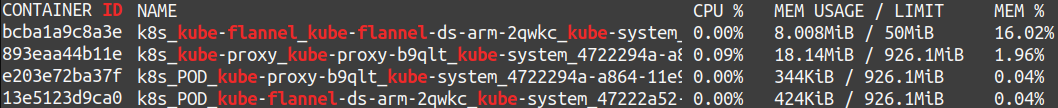
\includegraphics[scale=1.6]{figures/kubeContainerResourceUsageCut.png}
    \vspace*{-0.3cm}
    \caption{ The resource usage of Kubernetes containers.\\ The command used is \textit{docker stats | grep -E '(ID|kube|flannel)'}.}
    \label{fig:kubernetesResourceConsumptionCut}
\end{figure}
Most importantly, flannel and kube-proxy consume 0.86\% and 1.96\% of the memory, respectively\footnote{flannel's limit is 50MB, hence the 16.02\% in the figure.}. The CPU usage of all containers is negligible at below 1\%. Adding up the numbers, after the installation Kubernetes uses 7.7\% of the CPU and 11.7\% of the total memory. This translates to 0.43GHz CPU usage, see \cref{eq:cpuTotal}, and 108.35MB memory usage, see \cref{eq:ramTotal}.
\begin{equation} \label{eq:cpuTotal}
    1.4GHz * 4 \; \textrm{(cores)} * 0.077 = 0.4312GHz  \quad \textrm{(CPU usage)}
  \end{equation}
  \begin{equation} \label{eq:ramTotal}
    926.1MB * 0.117 = 108.3537MB  \quad \textrm{(RAM usage)}
  \end{equation}
Especially, the memory consumption is concerning as swap is disabled and thus a memory overflow could hinder the operating system from functioning correctly. 